\documentclass[10pt]{standalone}
\usepackage{amsmath}
\usepackage{pgf,tikz}
\usepackage{mathrsfs}
\usetikzlibrary{arrows}
\pagestyle{empty}
\begin{document}
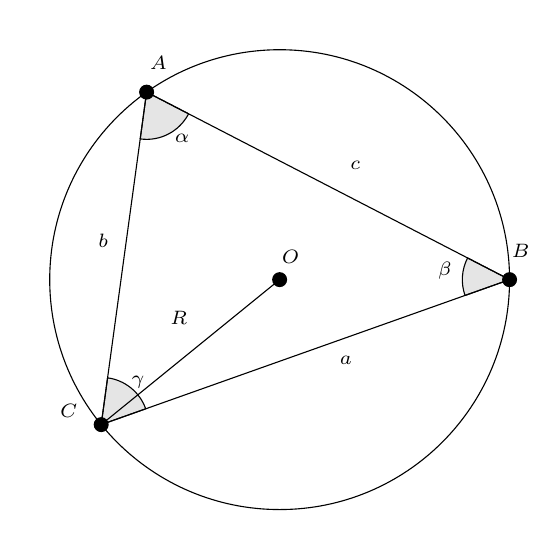
\begin{tikzpicture}[line cap=round,line join=round,>=triangle 45,x=1.0cm,y=1.0cm]
\clip(-3.2,-3.2) rectangle (3.2,3.2);
\draw [shift={(-1.689504537051402,2.3815907329519757)},color=black,fill=black,fill opacity=0.10000000149011612] (0,0) -- (-97.77709321493433:0.6) arc (-97.77709321493433:-27.324022658049074:0.6) -- cycle;
\draw [shift={(2.92,0.)},color=black,fill=black,fill opacity=0.10000000149011612] (0,0) -- (152.67597734195093:0.6) arc (152.67597734195093:199.54692944311472:0.6) -- cycle;
\draw [shift={(-2.266252880339495,-1.84133046527584)},color=black,fill=black,fill opacity=0.10000000149011612] (0,0) -- (19.546929443114752:0.6) arc (19.546929443114752:82.2229067850657:0.6) -- cycle;
\draw(0.,0.) circle (2.92cm);
\draw (-1.689504537051402,2.3815907329519757)-- (2.92,0.);
\draw (2.92,0.)-- (-2.266252880339495,-1.84133046527584);
\draw (-1.689504537051402,2.3815907329519757)-- (-2.266252880339495,-1.84133046527584);
\draw (0.,0.)-- (-2.266252880339495,-1.84133046527584);
\begin{scriptsize}
\draw [fill=black] (0.,0.) circle (2.5pt);
\draw[color=black] (0.14,0.29) node {$O$};
\draw [fill=black] (2.92,0.) circle (2.5pt);
\draw[color=black] (3.06,0.37) node {$B$};
\draw [fill=black] (-2.266252880339495,-1.84133046527584) circle (2.5pt);
\draw[color=black] (-2.68,-1.67) node {$C$};
\draw [fill=black] (-1.689504537051402,2.3815907329519757) circle (2.5pt);
\draw[color=black] (-1.54,2.75) node {$A$};
\draw[color=black] (0.96,1.45) node {$c$};
\draw[color=black] (0.84,-1.03) node {$a$};
\draw[color=black] (-2.24,0.49) node {$b$};
\draw[color=black] (-1.28,-0.49) node {$R$};
\draw[color=black] (-1.24,1.80) node {$\alpha$};
\draw[color=black] (2.1,0.11) node {$\beta$};
\draw[color=black] (-1.8,-1.3) node {$\gamma$};
\end{scriptsize}
\end{tikzpicture}
\end{document}